% Options for packages loaded elsewhere
\PassOptionsToPackage{unicode}{hyperref}
\PassOptionsToPackage{hyphens}{url}
%
\documentclass[
  ignorenonframetext,
]{beamer}
\usepackage{pgfpages}
\setbeamertemplate{caption}[numbered]
\setbeamertemplate{caption label separator}{: }
\setbeamercolor{caption name}{fg=normal text.fg}
\beamertemplatenavigationsymbolsempty
% Prevent slide breaks in the middle of a paragraph
\widowpenalties 1 10000
\raggedbottom
\setbeamertemplate{part page}{
  \centering
  \begin{beamercolorbox}[sep=16pt,center]{part title}
    \usebeamerfont{part title}\insertpart\par
  \end{beamercolorbox}
}
\setbeamertemplate{section page}{
  \centering
  \begin{beamercolorbox}[sep=12pt,center]{part title}
    \usebeamerfont{section title}\insertsection\par
  \end{beamercolorbox}
}
\setbeamertemplate{subsection page}{
  \centering
  \begin{beamercolorbox}[sep=8pt,center]{part title}
    \usebeamerfont{subsection title}\insertsubsection\par
  \end{beamercolorbox}
}
\AtBeginPart{
  \frame{\partpage}
}
\AtBeginSection{
  \ifbibliography
  \else
    \frame{\sectionpage}
  \fi
}
\AtBeginSubsection{
  \frame{\subsectionpage}
}

\usepackage{amsmath,amssymb}
\usepackage{iftex}
\ifPDFTeX
  \usepackage[T1]{fontenc}
  \usepackage[utf8]{inputenc}
  \usepackage{textcomp} % provide euro and other symbols
\else % if luatex or xetex
  \usepackage{unicode-math}
  \defaultfontfeatures{Scale=MatchLowercase}
  \defaultfontfeatures[\rmfamily]{Ligatures=TeX,Scale=1}
\fi
\usepackage{lmodern}
\ifPDFTeX\else  
    % xetex/luatex font selection
\fi
% Use upquote if available, for straight quotes in verbatim environments
\IfFileExists{upquote.sty}{\usepackage{upquote}}{}
\IfFileExists{microtype.sty}{% use microtype if available
  \usepackage[]{microtype}
  \UseMicrotypeSet[protrusion]{basicmath} % disable protrusion for tt fonts
}{}
\makeatletter
\@ifundefined{KOMAClassName}{% if non-KOMA class
  \IfFileExists{parskip.sty}{%
    \usepackage{parskip}
  }{% else
    \setlength{\parindent}{0pt}
    \setlength{\parskip}{6pt plus 2pt minus 1pt}}
}{% if KOMA class
  \KOMAoptions{parskip=half}}
\makeatother
\usepackage{xcolor}
\newif\ifbibliography
\setlength{\emergencystretch}{3em} % prevent overfull lines
\setcounter{secnumdepth}{-\maxdimen} % remove section numbering


\providecommand{\tightlist}{%
  \setlength{\itemsep}{0pt}\setlength{\parskip}{0pt}}\usepackage{longtable,booktabs,array}
\usepackage{calc} % for calculating minipage widths
\usepackage{caption}
% Make caption package work with longtable
\makeatletter
\def\fnum@table{\tablename~\thetable}
\makeatother
\usepackage{graphicx}
\makeatletter
\def\maxwidth{\ifdim\Gin@nat@width>\linewidth\linewidth\else\Gin@nat@width\fi}
\def\maxheight{\ifdim\Gin@nat@height>\textheight\textheight\else\Gin@nat@height\fi}
\makeatother
% Scale images if necessary, so that they will not overflow the page
% margins by default, and it is still possible to overwrite the defaults
% using explicit options in \includegraphics[width, height, ...]{}
\setkeys{Gin}{width=\maxwidth,height=\maxheight,keepaspectratio}
% Set default figure placement to htbp
\makeatletter
\def\fps@figure{htbp}
\makeatother

\makeatletter
\@ifpackageloaded{caption}{}{\usepackage{caption}}
\AtBeginDocument{%
\ifdefined\contentsname
  \renewcommand*\contentsname{Table of contents}
\else
  \newcommand\contentsname{Table of contents}
\fi
\ifdefined\listfigurename
  \renewcommand*\listfigurename{List of Figures}
\else
  \newcommand\listfigurename{List of Figures}
\fi
\ifdefined\listtablename
  \renewcommand*\listtablename{List of Tables}
\else
  \newcommand\listtablename{List of Tables}
\fi
\ifdefined\figurename
  \renewcommand*\figurename{Figure}
\else
  \newcommand\figurename{Figure}
\fi
\ifdefined\tablename
  \renewcommand*\tablename{Table}
\else
  \newcommand\tablename{Table}
\fi
}
\@ifpackageloaded{float}{}{\usepackage{float}}
\floatstyle{ruled}
\@ifundefined{c@chapter}{\newfloat{codelisting}{h}{lop}}{\newfloat{codelisting}{h}{lop}[chapter]}
\floatname{codelisting}{Listing}
\newcommand*\listoflistings{\listof{codelisting}{List of Listings}}
\makeatother
\makeatletter
\makeatother
\makeatletter
\@ifpackageloaded{caption}{}{\usepackage{caption}}
\@ifpackageloaded{subcaption}{}{\usepackage{subcaption}}
\makeatother
\ifLuaTeX
  \usepackage{selnolig}  % disable illegal ligatures
\fi
\usepackage{bookmark}

\IfFileExists{xurl.sty}{\usepackage{xurl}}{} % add URL line breaks if available
\urlstyle{same} % disable monospaced font for URLs
\hypersetup{
  pdftitle={Untitled},
  hidelinks,
  pdfcreator={LaTeX via pandoc}}

\title{Untitled}
\author{}
\date{}

\begin{document}
\frame{\titlepage}

\begin{frame}{Justification for studying REE.}
\phantomsection\label{justification-for-studying-ree.}
\begin{itemize}
\tightlist
\item
  Economics is about allocating resources efficiently.
\item
  To our understanding ``environment'' is also a scarce resource.
\end{itemize}
\end{frame}

\begin{frame}{What do we mean by ``environment''}
\phantomsection\label{what-do-we-mean-by-environment}
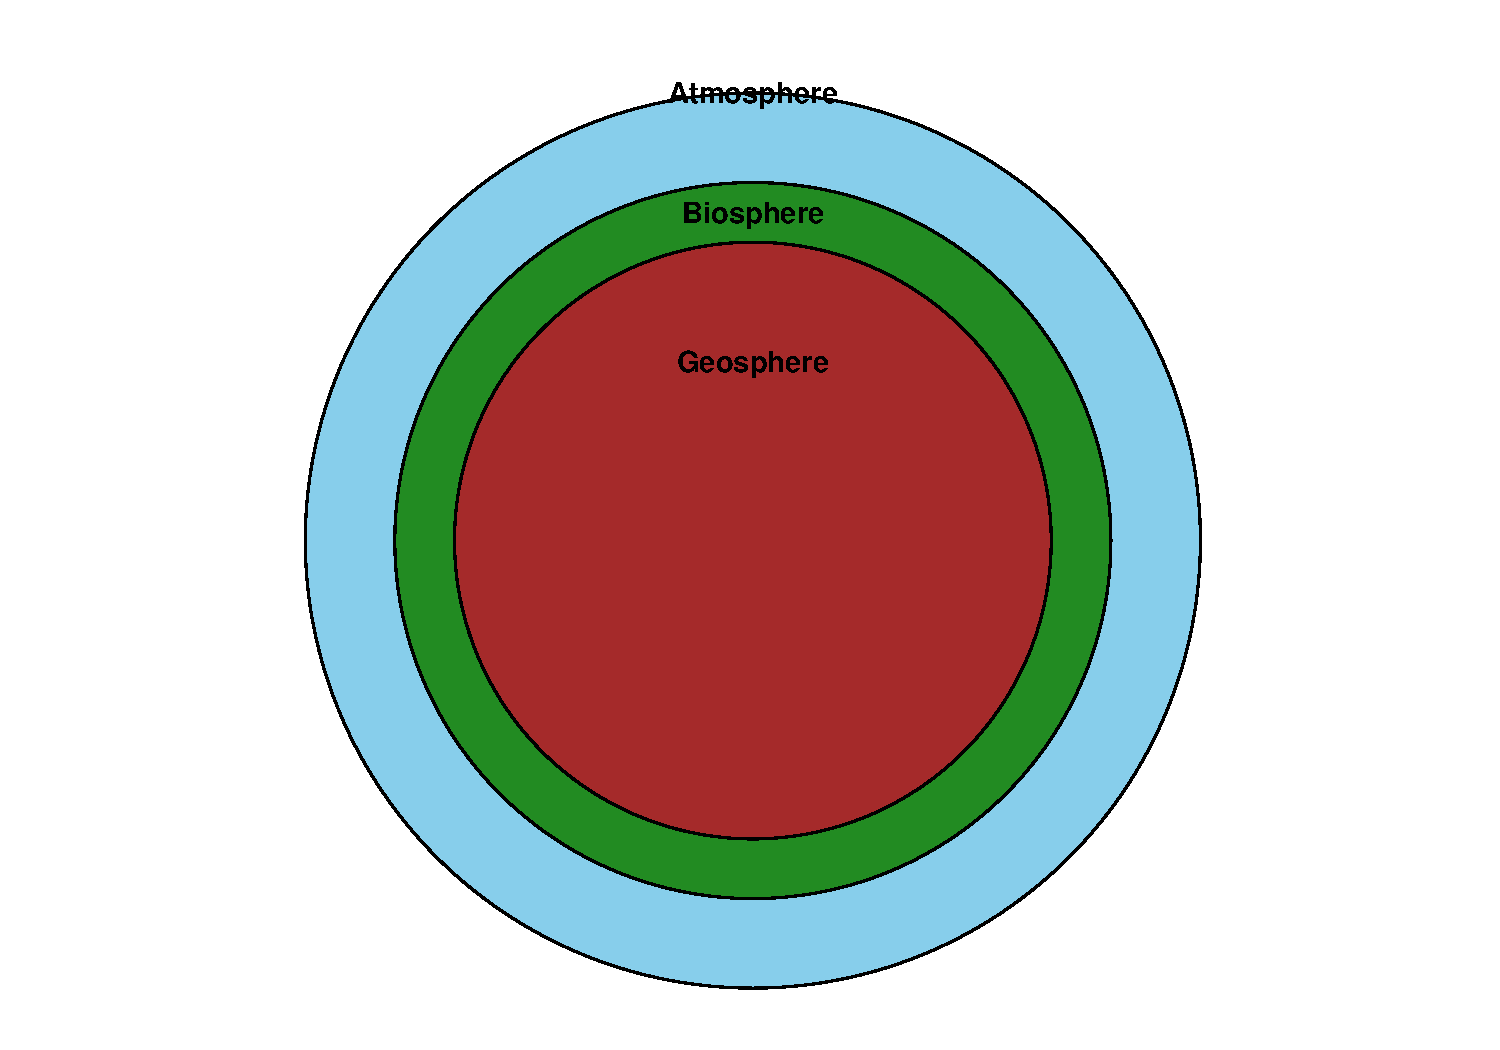
\includegraphics{intro_files/figure-beamer/unnamed-chunk-1-1.pdf}
\end{frame}

\begin{frame}{Definition of natural resource}
\phantomsection\label{definition-of-natural-resource}
\begin{itemize}
\item
  Naturally occurring resources which can be made available for mankind
  under feasible \textbf{social}, \textbf{economic}, and
  \textbf{technological} framework.- Can we classify sea water as a
  natural resource?
\item
  Two types:

  \begin{itemize}
  \tightlist
  \item
    Renewable Resources: Generating capacity - forests, fishery, solar
    energy, etc.
  \item
    Non-renewable resources: No generating capacity over an economically
    feasible time horizon - coal, oil, etc.
  \end{itemize}
\end{itemize}
\end{frame}

\begin{frame}
\begin{itemize}
\tightlist
\item
  Do renewable resources also get exhausted?

  \begin{itemize}
  \tightlist
  \item
    Yes, if the rate of extraction \(>\) the rate of growth.
  \end{itemize}
\item
  Are we exhausting our nonrenewable resources too rapidly or too
  slowly?

  \begin{itemize}
  \tightlist
  \item
    \textbf{Optimal rate of extraction}: The rate of extraction that
    maximises that inter-temporal benefits derived from such
    non-renewable resources.
  \end{itemize}
\end{itemize}
\end{frame}

\begin{frame}
\begin{itemize}
\tightlist
\item
  Example: 1000 kg of coal to be used over 10 years.
\end{itemize}

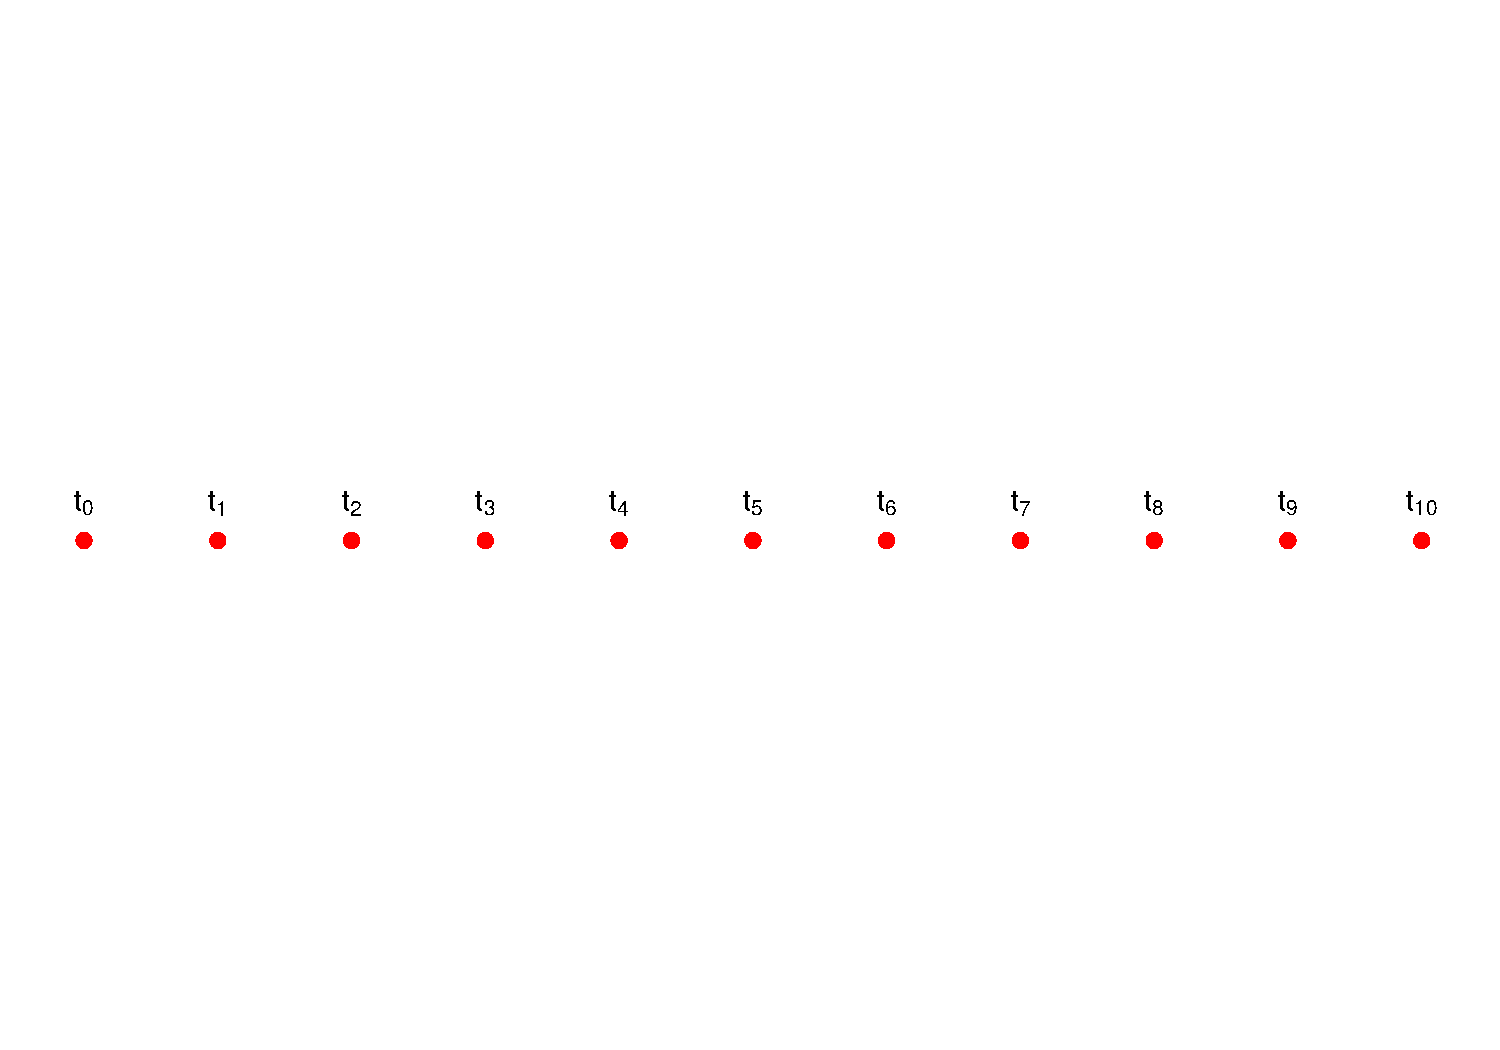
\includegraphics{intro_files/figure-beamer/unnamed-chunk-2-1.pdf}
\end{frame}

\begin{frame}{Natural resources as an open set}
\phantomsection\label{natural-resources-as-an-open-set}
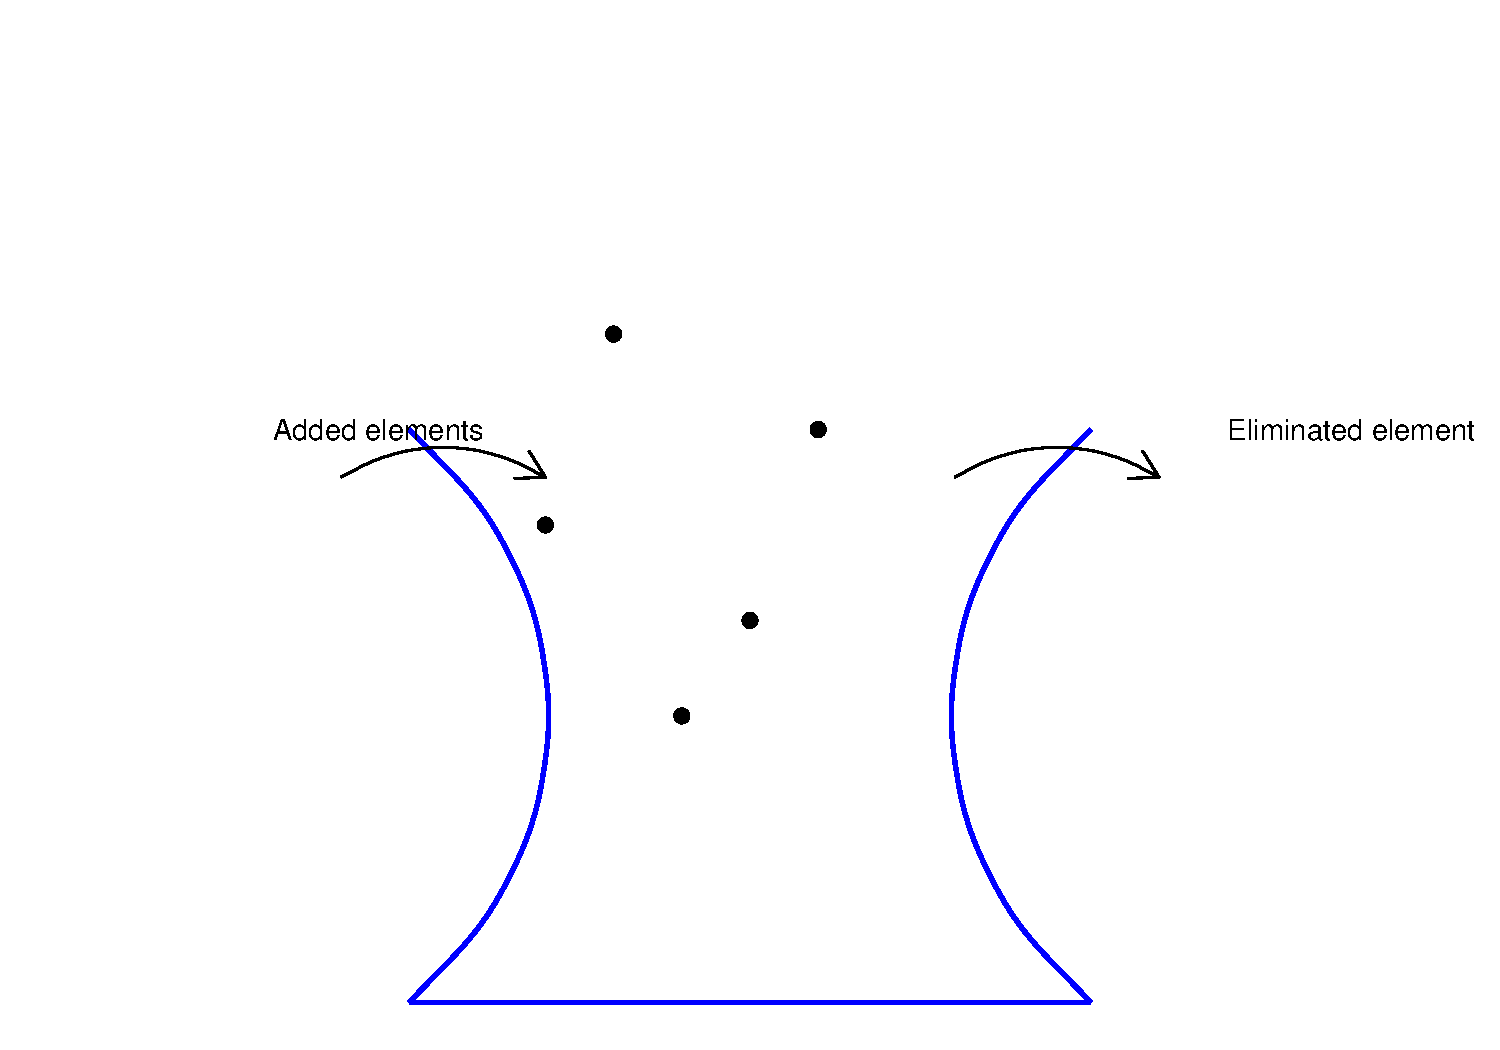
\includegraphics{intro_files/figure-beamer/unnamed-chunk-3-1.pdf}

\begin{itemize}
\tightlist
\item
  Added: Uranium
\item
  Eliminated: Extinct species of flora and fauna.
\end{itemize}
\end{frame}

\begin{frame}{The optimal path}
\phantomsection\label{the-optimal-path}
\begin{itemize}
\tightlist
\item
  What should be the optimal path (\emph{if we join the points we get a
  path}) of extraction for a non-renewable resource (NRR)?
\item
  For market goods

  \begin{itemize}
  \tightlist
  \item
    \(p = mc\), \(p\)- price , \(mc\)- marginal cost
  \end{itemize}
\end{itemize}
\end{frame}

\begin{frame}
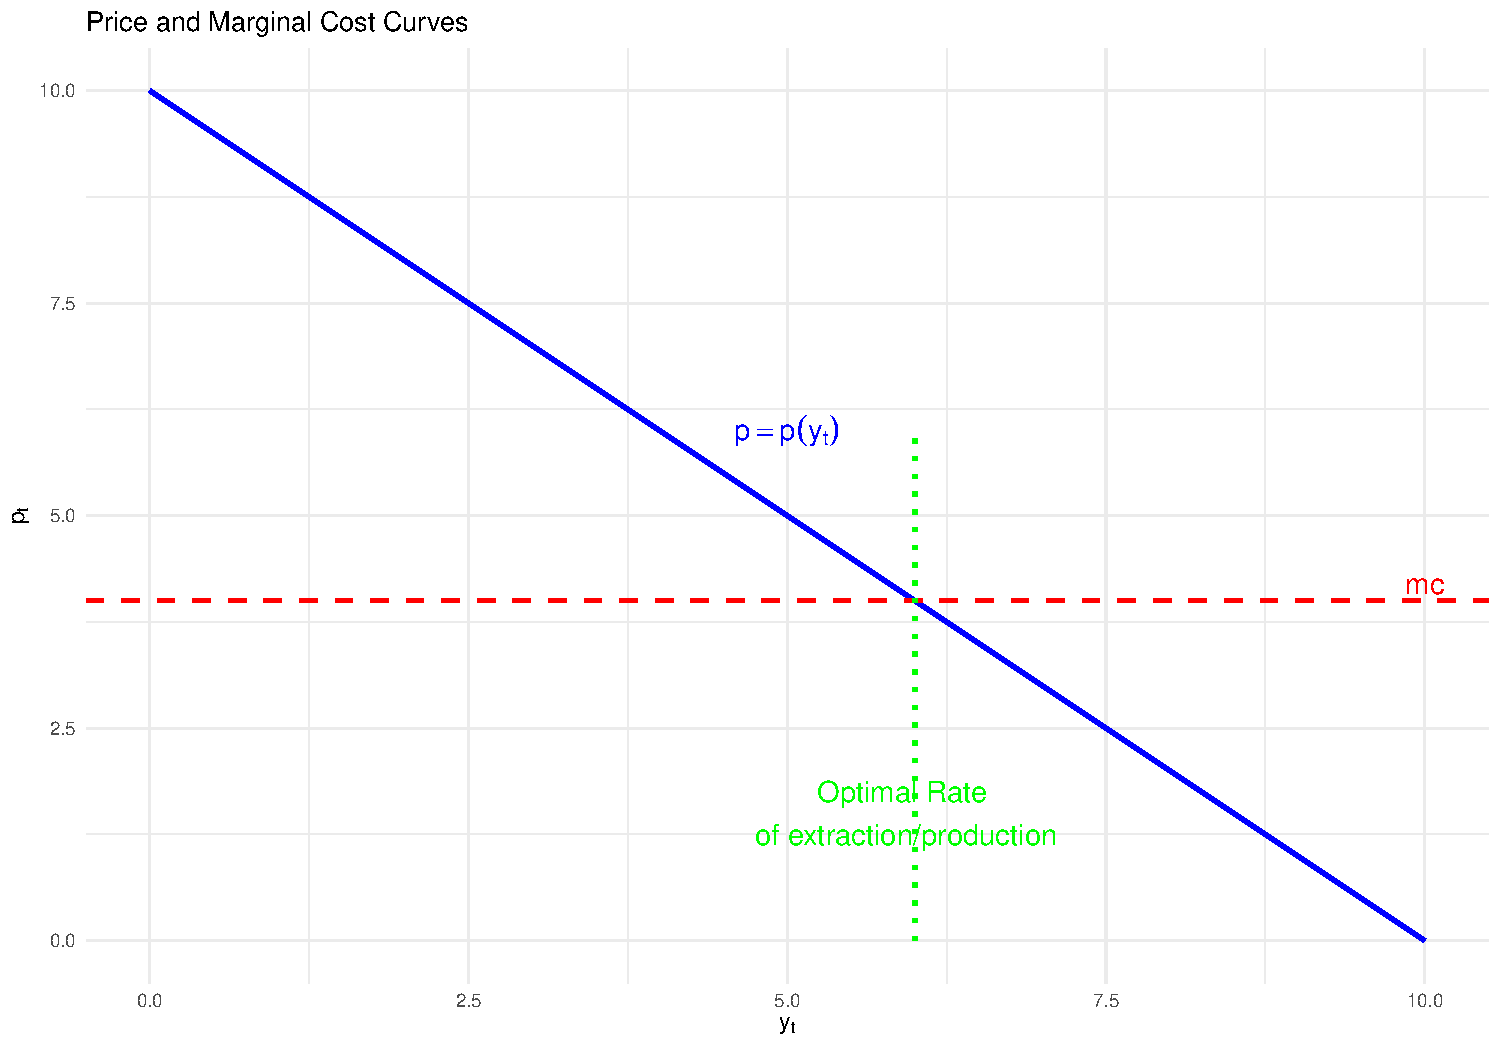
\includegraphics{intro_files/figure-beamer/unnamed-chunk-4-1.pdf}
\end{frame}

\begin{frame}[fragile]
\begin{itemize}
\tightlist
\item
  Can we apply \texttt{p\ =\ mc} for a NRR?

  \begin{itemize}
  \tightlist
  \item
    No, NRR are not easily replicable \(\rightarrow\) today's
    production/extraction has some opportunity cost as the \emph{same
    resource is not available for tomorrow.}
  \end{itemize}
\end{itemize}
\end{frame}

\begin{frame}
\begin{itemize}
\tightlist
\item
  In this situation we have an additional (opportunity) cost.
\end{itemize}

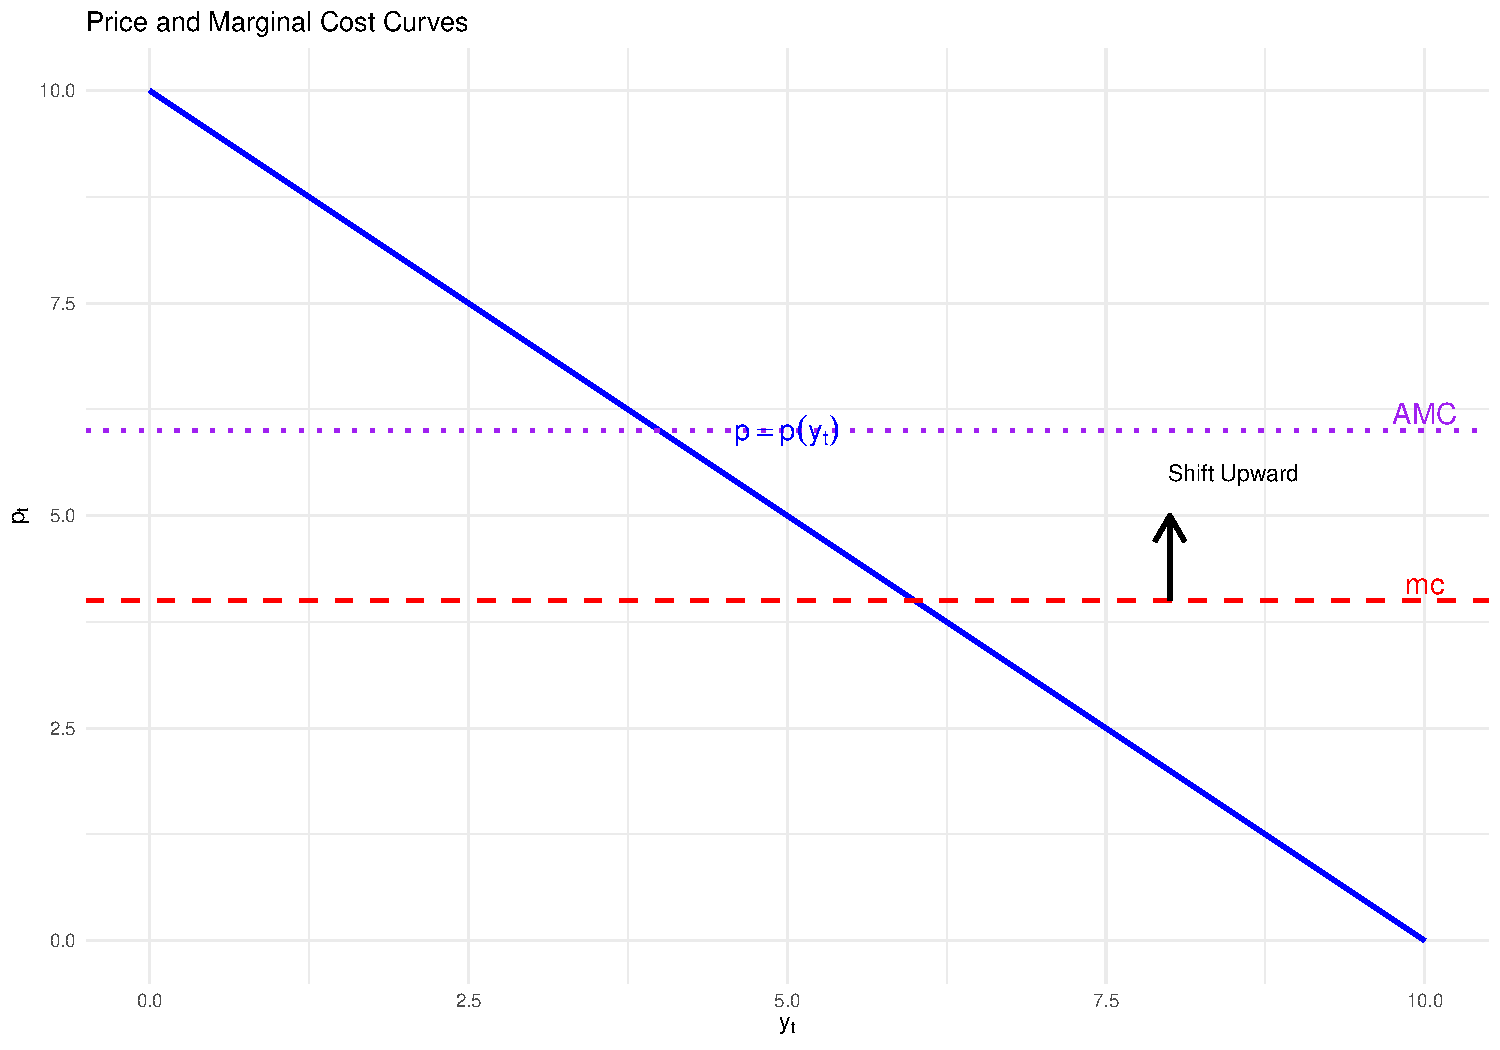
\includegraphics{intro_files/figure-beamer/unnamed-chunk-5-1.pdf}

\(p = mc_e + mu_c\) where; - \(mc_e:\) marginal cost of extraction -
\(mu_c:\) marginal user cost
\end{frame}

\begin{frame}
\begin{itemize}
\tightlist
\item
  Let us assume we have some amount of NRR which we are going to use in
  2 periods;

  \begin{itemize}
  \tightlist
  \item
    \(0: 1^{st} \text{period}\)
  \item
    \(1: \text{last period}\)
  \item
    \(p_0: \text{price at } t_0\)
  \item
    \(p_1: \text{price at } t_1\)
  \end{itemize}
\item
  The resource owner has to decide \textbf{whether to use the resource
  today or keep it for tomorrow}.

  \begin{itemize}
  \tightlist
  \item
    \(p_0 - mc_e\): Today's benefit
  \item
    \(p_1 - mc_e\): Tomorrow's benefit (if the resource is left for
    tomorrow)
  \end{itemize}
\end{itemize}
\end{frame}

\begin{frame}
\begin{itemize}
\tightlist
\item
  At \(t_0\), the owner has to convert tomorrow's benefit to today's
  benefit.
\item
  This benefit is given by \[
  \frac{p_1 - mc_e}{1 + r}
  \]
\end{itemize}

where \(r\) is the rate of interest or the discount rate.
\end{frame}

\begin{frame}{}
\phantomsection\label{section}
\begin{itemize}
\tightlist
\item
  We are converting tomorrow's benefit to today's benefit by discounting
  \emph{and the discount rate is \(r\)}.
\item
  If \((p_0 - mc_e) > \frac{(p_1 - mc_e)}{1 + r}\) \(\implies\) the
  resource owner should use it today. The RHS is also called the
  \textbf{discounted benefit}.
\item
  If \((p_0 - mc_e) < \frac{(p_1 - mc_e)}{1 + r}\) \(\implies\) the
  resource owner should use it tomorrow.
\item
  If \((p_0 - mc_e) = \frac{(p_1 - mc_e)}{1 + r}\) \(\implies\) the
  resource owner is indifferent between today's use and tomorrow's.
\end{itemize}
\end{frame}

\begin{frame}
\begin{itemize}
\tightlist
\item
  \((p_0 - mc_e) = \frac{(p_1 - mc_e)}{1 + r}\) is called the
  equilibrium condition.
\item
  \(p_0 = mc_e + \frac{(p_1 - mc_e)}{1 + r}\)
\item
  Since the marginal cost pricing is not applicable for NRR, an
  additional opportunity cost was added to \(mc_e\).
\item
  This component of cost is known as the marginal user cost (muc) where
  \(mu_c = \frac{(p_1 - mc_e)}{1 + r}\)
\item
  \(mc_e + mu_c = \text{augmented marginal cost}\)
\item
  If the \(mu_c\) is not added to the \(mc_e\) then the NRR may not be
  available for extraction tomorrow.
\end{itemize}
\end{frame}

\begin{frame}
\begin{align}
\because p_0 &= mc_e + \frac{(p_1 - mc_e)}{1 + r}\\
p_1 &= mc_e + (p_0 - mc_e)(1 + r) \\
p_2 &= mc_e + (p_0 - mc_e)(1 + r)^2\\
\text{In general we can write};\\
p_t &= mc_e + (p_0 - mc_e)(1 + r)^t\\
\end{align}

\begin{itemize}
\tightlist
\item
  This is the \textbf{price path} or a \textbf{series of optimal prices}
  for optimal extraction at various points in time.
\item
  This indicates that \(p_t\) is a \textbf{dynamic optimization} problem
  rather than a static optimization.
\end{itemize}
\end{frame}

\begin{frame}
\begin{align}
\because p_1 &= mc_e + (p_0 - mc_e)(1 + r) \\
(1+r) &= \frac{(p_1 - mc_e)}{(p_0 - mc_e)}  \\
r &= \frac{(p_1 - mc_e)-(p_0 - mc_e)}{(p_0 - mc_e)}
\end{align}

\begin{itemize}
\tightlist
\item
  This \(p - mc_e\) is also known as \textbf{Marginal Resource Rent}

  \begin{itemize}
  \tightlist
  \item
    where;
    \(p_1: \text{price of NRR}\\ mc_e: \text{cost of extraction of one unit of NRR}\\ r: \text{growth of marginal resource rent}\)
  \end{itemize}
\end{itemize}
\end{frame}

\begin{frame}
\begin{itemize}
\tightlist
\item
  We can now say that \emph{along the optimum path of marginal resource
  extraction, the marginal resource rent should grow at the rate of
  discount} i.e.~\(r = \frac{(p_1 - mc_e)-(p_0 - mc_e)}{(p_0 - mc_e)}\).
\item
  In other words; \emph{the most socially and economically profitable
  extraction path of a NRR is one along which marginal resource rent
  (MRR) must grow at the rate of interest or discount}:
  \textbf{Hotelling's Rule (1931)}.
\end{itemize}
\end{frame}

\begin{frame}
\begin{itemize}
\tightlist
\item
  Note that optimum extraction depends on two things
  \(p_1: \text{tomorrow's price }\) and
  \(r: \text{the discount or the interest rate}\)
\item
  \(p_1\) is the expected price that the resource owner will use.
\item
  \(r\) varies from person to person.

  \begin{itemize}
  \tightlist
  \item
    Bias for today then use heavy discount rate.
  \end{itemize}
\end{itemize}
\end{frame}

\begin{frame}
\begin{itemize}
\tightlist
\item
  We know that at equilibrium \(p_t = mc_e + (p_0 - mc_e)(1 + r)^t\).
\item
  Now \(\text{as }t \rightarrow \infty, p_t \rightarrow \infty\)
\item
  Is there any such possibility? For instance, say after 200 years or
  more the price of petrol becomes infinite.
\end{itemize}
\end{frame}

\begin{frame}
\begin{itemize}
\tightlist
\item
  The answer is \textbf{No}.
\end{itemize}

\begin{enumerate}
\tightlist
\item
  After 200 years or more we might find a substitute or an alternative
  resource or technology for petrol.
\end{enumerate}

\begin{itemize}
\tightlist
\item
  \textbf{Backstop}: The availability of alternative (substitute)
  resource (technology) which makes the utilization of existing resource
  more efficient. E.g. solar energy.
\end{itemize}

\begin{enumerate}
\setcounter{enumi}{1}
\tightlist
\item
  The availability of a backstop will impact (reduce) the demand for
  petrol and hence put a cap on the upper limit of the price.
\end{enumerate}
\end{frame}

\begin{frame}{Role of Backstop in determining the optimal price path of
an existing NRR}
\phantomsection\label{role-of-backstop-in-determining-the-optimal-price-path-of-an-existing-nrr}
\begin{itemize}
\tightlist
\item
  Let's assume \(mc_b\) is the marginal cost of extraction of the
  backstop, and \(mc_b > mc_e\)
\item
  We also assume that there is no user cost for the backstop (unlike the
  NRR) because we have just discovered the backstop and have it in
  adequate supply.
\end{itemize}
\end{frame}

\begin{frame}
\begin{itemize}
\tightlist
\item
  \textbf{Shift date}: the time at which the NRR gets exhausted.
\item
  Let us denote this as \(T\).
\item
  The price path of the existing NRR at time \(T\) is
\end{itemize}

\[
p_T = mc_e + (p_0 - mc_e)(1 + r)^T ... (1)
\] - Since there is no user cost for backstop, \[
\begin{align}
p_T = mc_b \ldots (2)\\
\text{where, } p_T:\text{price of the backstop}\\
\\
\text{From (1) and (2), we get}\\
mc_b &= mc_e + (p_0 - mc_e)(1+r)^T\\
p_0 - mc_e &= \frac{mc_b-mc_e}{(1+r)^T}
\end{align}
\]
\end{frame}

\begin{frame}
\end{frame}



\end{document}
